\documentclass[12pt]{article}
\usepackage[left=1in, right=1in, top=1in, bottom=1in]{geometry}
\usepackage{tikz}
\usepackage{setspace}
\usepackage{hyperref}
\usepackage{amsfonts, amssymb, amsmath} 
\usepackage[T1]{fontenc}
\usetikzlibrary{shadows.blur}
\usepackage{titlesec}

\author{Krisztián Szabó}
\date{Source: Contemporary Abstract Algebra by Joseph A. Gallian}
\renewcommand{\contentsname}{Content}

\titleformat{\section}[block]{\color{purple}\normalfont\Large\bfseries}{\thesection}{1em}{}
\title{\textcolor{purple}{\Huge\textbf{\textsc{Abstract algebra}}}}

\newcommand{\cent}[1]{\langle #1 \rangle}

\setlength{\parindent}{0pt}

\definecolor{modernyellow}{HTML}{F4E4BC}
\definecolor{moderngreen}{HTML}{BDDCBD}
\definecolor{colo}{HTML}{FFFC9B}

\tikzset{
	definition/.style={
		draw,
		fill=modernyellow, % Sárga színű keret a definíciókhoz
		line width=1pt,
		rounded corners, % Lekerekített szélek
		drop shadow={shadow blur steps=5,shadow xshift=1ex,shadow yshift=-1ex}, % Árnyék hozzáadása
		text width=0.9\textwidth, % Szöveg szélessége
		inner sep=10pt
	},
	corollary/.style={
		draw,
		fill=colo, % Zöld színű keret a tételekhez
		line width=1pt,
		rounded corners, % Lekerekített szélek
		drop shadow={shadow blur steps=5,shadow xshift=1ex,shadow yshift=-1ex}, % Árnyék hozzáadása
		text width=0.9\textwidth,
		inner sep=10pt
	},
	theorem/.style={
		draw,
		fill=moderngreen, % Zöld színű keret a tételekhez
		line width=1pt,
		rounded corners, % Lekerekített szélek
		drop shadow={shadow blur steps=5,shadow xshift=1ex,shadow yshift=-1ex}, % Árnyék hozzáadása
		text width=0.9\textwidth,
		inner sep=10pt
	},
	proof/.style={
		fill=white,
		rectangle,
		drop shadow={shadow blur steps=5,shadow xshift=1ex,shadow yshift=-1ex, moderngreen},
		%rounded corners=3pt,
		text width=0.9\textwidth,
		inner sep=6pt
	},
	proof1/.style={
		fill=white,
		rectangle,
		drop shadow={shadow blur steps=5,shadow xshift=1ex,shadow yshift=0, moderngreen},
		text width=0.9\textwidth,
		inner sep=6pt
	}
}

\begin{document}
	\maketitle
	\tableofcontents
	\newpage
	
	\section{Integers and Equivalence Relations}
	\subsection{Properties of integers}
	
	Much of abstract algebra involves properties of integers and sets. In this
	chapter we collect the properties we need for future reference.
	An important property of the integers, which we will often use, is the
	so-called \textit{Well ordering principle}. Since this property cannot be proved
	from the usual properties of arithmetic, we will take it as an axiom.
	
	\subsubsection{Well ordering principle}
	\begin{center}
		\textit{Every nonempty set of positive integers contains a smallest member}.
	\end{center}
	
	\subsubsection{Division algorithm}
	\tikz \node[theorem]
	{
		\textbf{Theorem.} Let $a$ and $b$ be integers with $b > 0$. Then there exists unique integers $q$ and $r$ with the property that $a = bq + r$, where $0 \leq r < b$.
	};\newline
	
	\tikz \node[proof]
	{
		\textbf{Proof.} We begin with the existence portion of the theorem. Consider the set $S = \{ a - bk \mid k \text{ is and integer and } a-bk \geq 0 \}$. If $0 \in S$, then $b$ divides $a$ and we may obtain the desired result with $q = \frac{a}{b}$ and $r = 0$. Now assume $0 \notin S$. Since $S$ is nonempty $\big( \text{if } a > 0, \, a-b \cdot 0 \in S; \, \text{if } a < 0, \, a-b(2a) = a(1-2b) \in S; \, a \neq 0 \text{ since } 0 \neq S \big)$, we may apply the Well ordering principle to conclude that $S$ has a smallest member, say $r = a-bq$. Then $a = bq + r$ and $r \geq 0$, so all that remains to be proved that $r < b$.\newline
		
		If $r \geq b$, then $a-b(q+1) = a-bq-b=r-b \geq 0$, so that $a-b(q+1) \in S$. But $a-b(q+1) < a-bq$, and $a-bq$ is the smallest member of $S$. So $r < b$.\newline
		
		To establish the uniqueness of $q$ and $r$, let us assume that there are integers $q, \, q', \, r$, and $r'$ such that
		\[
			a = bq + r, \quad 0 \leq r < b \quad \text{and} \quad a = bq' + r', \quad 0 \leq r' < b.
		\]
		For convenience, we may also suppose that $r' \geq r$. Then $bq + r = bq' + r'$ and $b(q-q') = r'-r$. So, $b$ divides $r'-r$ and $0 \leq r'-r \leq r' < b$. It follows that $r' - r = 0$.
	};
	
	\newpage
	\subsubsection{Greatest common divisor, relatively prime integers}
	\tikz \node[definition] 
	{
		\textbf{Definition.} The \textit{greatest common divisor} of two nonzero integers $a$ and $b$ is the largest of all common divisors of $a$ and $b$. We denote this integer by $gcd(a, \, b)$, when $gcd(a, \, b) = 1$, we say $a$ and $b$ are \textit{realively prime}.
	};
	
	\subsubsection{GCD is a linear combination}
	\tikz \node[theorem]
	{
		\textbf{Theorem.} For any nonzero integers $a$ and $b$, there exists integers $s$ and $t$ such that $gcd(a, \, b) = as + bt$. Moreover, $gcd(a, \, b)$ is the smallest positive integer of the form $as + bt$.
	};\newline
	
	\tikz \node[proof]
	{
		\textbf{Proof.} Consider the set $S = \{ am + bn \mid m, \, n \text{ are integeres and } am + bn > 0 \}$. Since $S$ is obviously nonempty, the Well ordering principle asserts that $S$ has a smallest member, say, $d = as + bt$. We claim that $d = gcd(a, \, b)$. To verify this claim, use the division algorithm to write $a = dq + r$, where $0 \leq r < d$. If $r > 0$, then $r = a-dq = a-(as+bt)q=a-asq-btq=a(1-sq)+b(-tq) \in S$, contradicting the fact that $d$ is the smallest member of $S$.\newline
		
		So, $r = 0$ and $d$ divides a. Analogously (or, better yet, by symmetry), $d$ divides $b$ as well. This proves that $d$ is a common divisor of $a$ and $b$. Now suppose $d'$ is another common divisor of $a$ nad $b$ and write $a = d'h$ and $b = d'k$. Then $d = as + bt = (d'h)s + (d'k)t = d'(hs + kt)$, so that $d'$ is a divisor of $d$. Thus, among all common divisors of $a$ and $b$, $d$ is the greatest.
	};\newline
	
	
	\tikz \node[theorem]
	{
		\textbf{Corollary.} If $a$ and $b$ are relatively prime, than there exist integers $s$ and $t$ such that $as + bt = 1$.
	};
	
	\subsubsection{Euclid's lemma}
	\tikz \node[theorem]
	{
		\textbf{Lemma.} If $p$ is is prime that divides $ab$, then $p$ divides $a$ or $p$ divides $b$.
	};\newline
	
	\tikz \node[proof]
	{
		\textbf{Proof.} Suppose $p$ is a prime that divides $ab$ but does not divide $a$. We must show that $p$ divides $b$. Since $p$ does not divide $a$, ther are integers $s$ and $t$ such that $1 = as + pt$. Then $b = abs + ptb$. and since $p$ divides the right-hand side of the equation, $p$ also divides $b$.
	};
		
	\subsubsection{Fundamental theorem of arithmetic}
	\tikz \node[theorem]
	{
		\textbf{Theorem.} Every integer greater than $1$ is a prime or a product of primes. This product is unique, except the order in which the factors appear. That is, if $n = p_1p_2 \cdots p_r$ and $n = q_1q_2 \cdots q_s$, where the $p$'s and $q$'s are primes, then $r = s$ and, after renumbering the $q$'s, we have $p_i = q_i$ for all $i$.
	};\newline
	
	\tikz \node[proof]
	{
		\textbf{Proof.} Later.
	};
	
	
	\subsubsection{Least common multiple}
	\tikz \node[definition]
	{
		\textbf{Definition.} The \textit{least common multiple} of two nonzero integers $a$ and $b$ is the smallest positive integer that is a multiple of both $a$ and $b$. We will denote this integer by $lcm(a, \, b)$.
	};
	
	\subsection{Mathematical induction}
	\subsubsection{Fist principle of mathematical induction}
	\tikz \node[theorem]
	{
		\textbf{Theorem.} Let $S$ be a set of integers containing $a$. Suppose $S$ has the property that whenever some integer $n \geq a$ belongs to $S$, then the integer $n+1$ also belongs to S. Then, S contains every integer greater than or equal to $a$.
	};\newline
	
	\tikz \node[proof]
	{
		\textbf{Proof.} $S$ contains $a$. But if $S$ contains an element $n \geq a$, then $n + 1$ is also in $S$. So $a + 1$ is also in $S$. But $S$ contains the element $a + 1$, so $a + 2$ is also in $S$. This gives us the result, that $S$ contains all the integers greater than or equal to $a$. 
	};
	
	\subsubsection{Second principle of mathematical induction}
	\tikz \node[theorem]
	{
		\textbf{Theorem.} Let $S$ be a set of integers containing $a$. Suppose $S$ has the property that $n$ belongs to $S$ whenever every integer less then $n$ and greater than or equal to $a$ belongs to $S$. Then, $S$ contains every integer greater than or equal to $a$.
	};\newline
	
	\tikz \node[proof]
	{
		\textbf{Proof.} $S$ contains $a$. Let $n_1$ be $a + 1$. All the numbers that are less than $n_1$ and greater than or equal to $a$ is only $a$, and it is in $S$, so $a + 1$ is also in $S$. Let $n_2$ be $a + 2$. The numbers that are less than $n_2$ and greater than or equal to $a$ are $n_2 = a + 2 > n_1 = a + 1 > a \geq a$. So $n_2$ is also in $S$. This, again gives us the result that all the integers that are greater than or equal to $a$ are in $S$.
	};\newline
	
	To use this form of induction, we first show that the statement is true for the integer $a$. We then assume that the statement is true for all integers that are greater than or equal to $a$ and less then $n$, and use this assumption to prove that the statement is true for $n$.\newline
	
	\textbf{Clarity.} So what have just we proven? We prooved that \textbf{if} all integers that are less than $n$ and greater than or equal to $a$ are in $S$, \textbf{then} $n$ is also in $S$. And most importantly, $a$ is also in $S$. Look at $a + 1$, the first half holds, because $a$ is in $S$, so $a + 1$ must be in $S$. Look at $a + 2 \dots$
	
	
	\subsection{Equivalence relations}
	\subsubsection{Equivalence relation}
	\tikz \node[definition]
	{
		\textbf{Definition.} An \textit{equivalence relation} on a set $S$ is a set $R$ of ordered pairs of elements of $S$ such that
		\begin{enumerate}
			\item $(a, \, a) \in R$ for all $a \in S$ (reflexive property).
			\item $(a, \, b) \in R$ implies $(b, \, a) \in R$ (symmetric property).
			\item $(a, \, b) \in R$ and $(b, \, c) \in R$ imply $(a, \, c) \in R$ (transitive property).
		\end{enumerate}
	};\newline
	
	When $R$ is an equivalence relation on a set $S$, it is customary to write $aRb$ instead of $(a, \, b) \in R$. Also, since an equivalence relation is just a generalization of equality, a suggestive symbol such as $\approx$, $\equiv$, $\thicksim$. Using this notation, the three conditions for an equivalence relation become $a \thicksim a; \, a \thicksim b$ implies $b \thicksim a$; and $a \thicksim b$ and $b \thicksim c$ imply $a \thicksim c$. If $\thicksim$ is an equivalence relation on a set $S$ and $a \in S$, then the set $[a] = \{ x \in S \mid x \thicksim a \}$ is called the equivalence class of $S$ containing $a$.\newline
	
	\textbf{Example.} Let $S$ be the set of \textbf{all} polynomials with the real coefficients. If $f, \, g \in S$ define $f \thicksim g$ if $f' = g'$, where $f'$ is the derivative of $f$. Then, $\thicksim$ is an equivalence relation on $S$. Since two polynomials with equal derivatives differ by a constant, we see that for any $f$ in $S$, $[f] = \{ f + c \mid c \text{ is real} \}$.\newline
	
	\textbf{Example.} Let $S$ be the set of integers and let $n$ be a positive integer. If $a, \, b \in S$, define $a \equiv b$ if $a$ mod $n = b$ mod $n$. (that is, if $a-b$ is divisible by $n$). Then, $\equiv$ is an equivalence relation on $S$. and $[a] = \{ a + kn \mid k \in S \}$. Since this particular relation is important in abstract algebra, we will take the trouble to verify that it is indeed an equivalence relation. Certainly, $a - a$ is divisible by $n$, so that $a \equiv a$ for all $a$ in $S$. Next, assume that $a \equiv b$, say, $a - b = rn$. Then $b - a = (-r)n$, and therefore $b \equiv a$. Finally, assume that $a \equiv b$ and $b \equiv c$, say $a-b = rn$ and $b-c = sn$. Then, we have $a - c = (a-b)+(b-c)=rn+sn=(r+s)n$, so that $a \equiv c$.
	
	\newpage
	\subsubsection{Partition}
	\tikz \node[definition]
	{
		\textbf{Definition.} A \textit{partition} of a set $S$ is a collection of nonempty disjoint subsets of $S$ whose union is $S$.
	};
	
	\subsubsection{Equivalence classes partition}
	\tikz \node[theorem]
	{
		\textbf{Theorem.} The equivalence classes of an equivalence relation on a set $S$ constitute a partition of $S$. Conversely, for any partition $P$ of $S$, there is an equivalence relation on $S$ whose equivalence classes are the element of $P$.
	};\newline
	
	\tikz \node[proof]
	{
		\textbf{Proof.} Let $\thicksim$ be an equivalence relation on a set $S$. For any $a \in S$, the reflexive property shows that $a \in [a]$. So, $[a]$ is a nonempty and the union of all equivalence classes is $S$. Now, suppose that $[a]$ and $[b]$ are distinct equivalence classes. We must show that $[a] \cap [b] = \emptyset$. On the contrary, assume $c \in [a] \cap [b]$. We will show that $[a] \subseteq [b]$. To this end, let $x \in [a]$. We then have $c \thicksim a, \, c \thicksim b$, and $x \thicksim a$. By the symmetric property, we also have $a \thicksim c$. Thus, by transitivity, $x \thicksim c$, and transitivity again, $x \thicksim b$. This proves $[a] \subseteq [b]$. Analogously, $[b] \subseteq [a]$. Thus, $[a] = [b]$, in contradiction to our assumption that $[a]$ and $[b]$ are distinc equivalence classes. \newline
		
		To prove the converse, let $P$ be a collection of nonempty disjoint subsets of $S$ whose union is $S$. Define $a \thicksim b$ if $a$ and $b$ belong to the same subset in the collection.
	};\newpage
	
	\subsection{Functions (mappings)}
	
	Although the concept of a function plays a central role in nearly every
	branch of mathematics, the terminology and notation associated with
	functions vary quite a bit. In this section, we establish ours.
	
	\subsubsection{Function (mapping)}
	\tikz \node[definition]
	{
		\textbf{Definition.} A \textit{function} (or mapping) $\phi$ from a set $A$ to a set $B$ is a rule that assigns to each element $a$ of $A$ exactly one element $b$ of $B$. The set $A$ is called the \textit{domain} of $\phi$, and $B$ is called the \textit{range} of $\phi$. If $\phi$ assigns $b$ to $a$, then $b$ is called the \textit{image of $a$ under $\phi$}. The subset of $B$ comprising all the images of elements of $A$ is called the \textit{image of $A$ under $\phi$}.
	};\newline
	
	We use the shorthand $\phi : A \to B$ to mean that $\phi$ is a mapping from $A$ to $B$. We will write $\phi(a) = b$ or $\phi : a \to b$ indicate that $\phi$ carries $a$ to $b$.
	
	\subsubsection{Composition of functions}
	\tikz \node[definition]
	{
		\textbf{Definition.} Let $\phi : A \to B$ and $\psi : B \to C$. The \textit{composition} $\psi\phi$ is the mapping from $A$ to $C$ defines by $(\psi\phi)(a) = \psi(\phi(a))$ for all $a$ in $A$.
	};
	
	\subsubsection{One-to-one function}
	\tikz \node[definition]
	{
		\textbf{Definition.} A function $\phi$ from a set $A$ is called \textit{one-to-one} if for every $a_1, \, a_2 \in A$, $\phi(a_1) = \phi(a_2)$ implies $a_1 = a_2$.
	};
	
	\subsubsection{Function from $A$ onto $B$}
	\tikz \node[definition]
	{
		\textbf{Definition.} A function $\phi$ from $A$ to a set $B$ is said to be \textit{onto} $B$ if each element of $B$ is the image of at least one element of $A$. In symbols, $\phi : A \to B$ is onto if for each $b$ in $B$ there is at least one $a$ in $A$ such that $\phi(a) = b$.
	};
	
	\subsubsection{Properties of functions}
	\tikz \node[theorem]
	{
		\textbf{Theorem.} Given functions $\alpha : A \to B, \, \beta : B \to C$, and $\gamma: C \to D$, then
		\begin{enumerate}
			\item $\gamma(\beta\alpha) = (\gamma\beta)\alpha$ (associativity).
			\item If $\alpha$ and $\beta$ are one-to-one, then $\beta\alpha$ is one-to-one.
			\item If $\alpha$ and $B$ are onto, then $\beta\alpha$ is onto.
			\item If $\alpha$ is one-to-one and oneto, then there is a function $\alpha^{-1}$ from $B$ onto $A$ such that $(\alpha^{-1}\alpha)(a) = a$ for all $a$ in $A$ and $(\alpha\alpha^{-1})(b) = b$ for all $b$ in $B$.
		\end{enumerate}
	};\newline
	
	\tikz \node[proof]
	{
		\textbf{Proof.} we prove only part 1. The remaining parts are left as exercises. Let $a \in A$. Then $(\gamma(\beta\alpha))(a) = \gamma((\beta\alpha)(a)) = \gamma(\beta(\alpha(a)))$ On the other hand, $((\gamma\beta)\alpha)(a) = (\gamma\beta)(\alpha(a)) = \gamma(\beta(\alpha(a))).$
	};
	
	\newpage
	
	
	
	\section{Groups}
	\subsection{Definition of groups}
	
	The term \textit{group} was used by Galois around 1830 to describe sets of
	one-to-one functions on finite sets that could be grouped together to
	form a set closed under composition. As is the case with most fundamental
	concepts in mathematics, the modern definition of a group that
	follows is the result of a long evolutionary process. Although this definition
	was given by both Heinrich Weber and Walter von Dyck in 1882,
	it did not gain universal acceptance until the 20th century.
	
	\subsubsection{Binary operation}
	\tikz \node[definition]
	{
		\textbf{Definition.} Let $G$ be a set. A binary operation on $G$ is a function that assigns each ordered pair of elements of G an element of G.
	};\newline
	
	\subsubsection{Group}
	\tikz \node[definition]
	{
		Let $G$ be a set together with a binary operation (usually called multiplication) that assigns to each ordered pair $(a, \, b)$ of elements of $G$ an element in $G$ denoted by $ab$. We say $G$ is a \textbf{group} under this operation if the following three properties are satisfied.
		\begin{enumerate}
			\item \textit{Associativity}. The operation is associative; that is, $(ab)c = a(bc)$ for all $a, \, b, \, c$ in $G$.
			\item \textit{Identity.} There is an element $e$ (called \textit{identity}) in $G$ such that $ae = ea = a$ for all $a$ in $G$.
			\item \textit{Inverses.} For each element $a$ in $G$, there is an element $b$ in $G$ (called an \textbf{inverse} of $a$) such that $ab = ba = e$.
		\end{enumerate}
	};\newline
	
	If a group has the property that $ab = ba$ for every pair of elements $a$ and $b$, we say the group is \textit{Abelian}.
	
	\subsection{Elementary properties of groups}
	\subsubsection{Uniqueness of the identity}
	\tikz \node[theorem]
	{
		\textbf{Theorem.} In a group $G$, there is only one identity element.
	};\newline
	
	\tikz \node[proof]
	{
		\textbf{Proof.} Suppose both $e$ and $e'$ are indentities of $G$. Then,
		\begin{enumerate}
			\item $ae = a$ for all $a$ in $G$, and
			\item $e'a = a$ for all $a$ in $G$.
		\end{enumerate}
		The choices of $a = e'$ in $1.$ and $a = e$ in $2.$ yield $e'e = e'$ and $e'e = e$. Thus, $e$ and $e'$ are both equal to $e'e$ and so are equal to each other.
	};
	
	\subsection{Cancellation}
	\tikz \node[theorem]
	{
		\textbf{Theorem.} In a group $G$, the right and left cancellation laws hold; that is, $ba = ca$ implies $b = c$, and $ab = ac$ implies $b = c$.
	};\newline
	
	\tikz \node[proof]
	{
		\textbf{Proof.} Suppose $ba = ca$. Let $a'$ be an inverse of $a$. Then, muliplying on the right by $a'$ yields $(ba)a' = (ca)a'$. Associativity yields $b(aa') = c(aa')$. Then, $be = ce$ and, therefore, $b = c$ as desired. Simirarly, one can prove that $ab = ac$ implies $b = c$ by multiplying by $a'$ on the left.
	};
	
	\subsubsection{Uniqueness of inverses}
	\tikz \node[theorem]
	{
		\textbf{Theorem.} For each element $a$ in a group $G$, there is a unique element $b$ in $G$ such that $ab = ba = e$.
	};\newline
	
	\tikz \node[proof]
	{
		\textbf{Proof.} Suppose $b$ and $c$ are both inverses of $a$. Then $ab = e$ and $ac = e$, so that $ab = ac$. Canceling the $a$ on both sides gives $b = c$, as desired.
	};\newline
	
	We may unambiguously denote it by $g^{-1}$. This notation is suggested by that used for ordinary real numbers under multiplication. Similarly, when $n$ is a positive integer, the associative law allows us to use $g^n$ to deont the unambiguous product
	\[
		\underbrace{gg\cdots g.}_{n \text{ factors}}
	\]
	We define $g^0 = e$. When $n$ is negative, we define $g^n = (g^{-1})^{|n|}$ . Unlike for real numbers, in an abstract algebra group we do not permit noninteger exponents such as $g^{1/2}$. With this notation, the familiar laws of exponents hold for groups; that is, for all integers $m$ and $n$ and any group element $g$, we have $g^mg^n = g^{m+n}$ and $(g^m)^n = g^{mn}$. Although the laws of exponents fail to hold for expressions involving two group elements. Thus, for groups in general, $(ab)^n \neq a^nb^b$.\newline
	Also, one must be careful with this notation when dealing with a specific group whose binary operation is addition and is denoted by $"+"$. In this case, the definitions and group properties expressed in multiplicative notation must be translated to additive notation. For example, the inverse of $g$ is written as $-g$. Likewise, for example, $g^3$ means $g + g + g$ and is usually written as $3g$, whereas $g^{-3}$ means $(-g) + (-g) + (-g)$.
	
	\subsubsection{Socks-shoes property}
	\tikz \node[theorem]
	{
		\textbf{Theorem.} For group elements $a$ and $b$, $(ab)^{-1} = b^{-1}a^{-1}$.
	};\newline
	
	\tikz \node[proof]
	{
		\textbf{Proof.} Since $(ab)(ab)^-1 = e$ and $(ab)(b^{-1}a^{-1}) = a(bb^{-1})a^{-1} = aea^{-1} = aa^{-1} = e$, we have by the theorem of uniqueness of inverses that $(ab)^-1 = b^{-1}a^{-1}$.
	};
	
	\newpage
	\section{Finite groups; subgroups}
	\subsection{Terminology and notation}
	As we will soon discover, finite groups - that is, groups with finitely many elements - have interesting arithmetic properties. To faciliate the study of finite groups, it is convenient to introduce some terminology and notation.
	
	\subsubsection{Order of a group}
	\tikz \node[definition]
	{
		\textbf{Definition.} The number of elements of a group (finite or infinite) is called its \textit{order}. We will use $|G|$ to denote the order of $G$.
	};\newline
	
	Thus, the group $Z$ of integers under addition has infinite order, whereas the group $U(10) = \{ 1,3,5,7 \}$ under multiplication modulo $10$ has order $4$.
	
	\subsubsection{Order of an element}
	\tikz \node[definition]
	{
		\textbf{Definition.} The \textit{order} of an element $g$ in a group $G$ is the smallest positive integer $n$ such that $g^n = e$. (In additive notation, this would be $ng = 0$.) If no such integer exists, we say that $g$ has \textit{infinite order}. The order of an element $g$ is denoted by $|g|$.
	};\newline
	
	So, to find the order of a group element $g$, you need only compute the sequence of products $g, \, g^2, \, g^3, \, \dots$, until you reach the indentity for the first time. The exponenet of this product (or coefficient if the operation is addition) is the order of $g$. If the indentity never appears in the sequence, then $g$ has infinite order.
	
	\subsubsection{Subgroup}
	\tikz \node[definition]
	{
		\textbf{Definition.} If a subset $H$ of a group $G$ is itself a group under the operation of $G$, we say that $H$ is a \textit{subgroup} of $G$.
	};\newline
	
	We use the notation $H \leq G$ to mean that $H$ is a subgroup of $G$. If we want to indicate that $H$ is a subgroup of $G$ but is not equal to $G$ itself, we write $H < G$. Such a subgroup is called a \textit{proper subgroup}. The subgroup $\{ e \}$ is called the \textit{trivial subgroup} of $G$; a subgroup that is not $\{ e\}$ is called a \textit{nontrivial subgroup} of $G$.\newline
	Notice that $Z_n$ under addition modulo $n$ is not a subgroup of $Z$ under addition, since addition modulo $n$ is not the operation of $Z$.
	
	\subsection{Subgroup tests}
	When determining whether or not a subset $H$ of a group $G$ is a subgroup of $G$, one need not directly verify the group axioms. The next three results provide simple tests that suffice to show that a subset of a group is a subgroup.
	
	\subsubsection{One-step subgroup test}
	\tikz \node[theorem]
	{
		\textbf{Theorem.} Let $G$ be a group and $H$ a nonempty subset of $G$. If $ab^{-1}$ is in $H$ whenever $a$ and $b$ are in $H$, then $H$ is a subgroup of $G$. (In additive notation, if $a-b$ is in $H$ whenever $a$ and $b$ are in $H$, then $H$, is a subgroup of $G$.)\newline
		
		\textit{Meaning of whenever: if $a$ and $b$ are in $H$, then $ab^{-1}$ is also in $H$.}
	};\newline
	
	\tikz \node[proof]
	{
		\textbf{Proof.} Since the operation of $H$ is the same as that of $G$, it is clear that this operation is associative. Next, we show that $e$ is in $H$. Since $H$ is nonempty, we may pick some $x$ in $H$. Then, letting $a = x$ and $b = x$ in the hypothesis, we have $e = xx^{-1} = ab^{-1}$ is in $H$. To verify that $x^{-1}$ is in $H$ whenever $x$ is in $H$, all we need to do is choose $a = e$ and $b = x$ in the statement of the theorem. Finally, the proof will be complete when we show that $H$ is closed; that is, if $x, \, y$ belong to $H$, we must show that $xy$ is in $H$ also. Well, we have already shown that $y^{-1}$ is in $H$ whenever $y$ is; so, letting $a = x$ and $b = y^{-1}$, we have $xy = x(y^{-1})^{-1} = ab^{-1}$ is in $H$.
	};\newline
	
	There are actually four steps involved in applying the theorem. Notice the similarity between the last three steps listed below and the three steps involved in the Principle of the mathematical induction.
	
	\begin{enumerate}
		\item Identify the property $P$ that distinguishes the elements of $H$; that is, identify a defining condition.
		\item Prove that the identity has property $P$. (This verifies that $H$ is nonempty.)
		\item \textit{Assume} that two elements $a$ and $b$ have property $P$.
		\item Use the assumption that $a$ and $b$ have property $P$ to show that $ab^{-1}$ has property $P$.
	\end{enumerate}
	
	\textbf{Example.} Let $G$ be an Abelian group with identity $e$. Then $H = \{x \in G \mid x^2 = e\}$ is a subgroup of $G$. Here, the defining property of $H$ is the condifiton $x^2=e$. So, we first note that $e^2 = e$, so that $H$ is nonempty. Now assume that $a$ and $b$ belong to $H$. This means $a^2 = b^2 = e$. Finally, we must show that $(ab^{-1})^2 = e$. Since $G$ is Abelian, $(ab^{-1})^2 = ab^{-1}ab^{-1} = a^2(b^{-1})^2 = a^2(b^2)^{-1} = ee^{-1} = e.$ Therefore, $ab^{-1}$ belongs to $H$ and, by the One-step subgroup test, $H$ is a subgroup of $G$.
	
	\subsubsection{Two-step subgroup test}
	\tikz \node[theorem]
	{
		\textbf{Theorem.} Let $G$ be a group and let $H$ be a nonempty subset of $G$. If $ab$ is in $H$ whenever $a$ and $b$ are in $H$ ($H$ is closed under the operation), and $a^{-1}$ is in $H$ ($H$ is closed under taking inverses), then $H$ is a subgroup of $G$.
	};\newline
	
	\tikz \node[proof]
	{
		\textbf{Proof.} By the One-step subgroup test theorem, it suffices to show that $a, \, b \in H$ implies $ab^{-1} \in H$. So, we suppose that $a, \, b \in H$. Since $H$ is closed under taking inverses, we also have $b^{-1} \in H$. This, $ab^{-1} \in H$ by closure under multiplication.
	};\newline
	
	When dealing with finite groups, it is easier to use the following subgroup test.
	
	\subsubsection{Finite subgroup test}
	\tikz \node[theorem]
	{
		\textbf{Theorem.} Let $H$ be a nonempty finite subset of a group $G$. If $H$ is closed under the operation of $G$, then $H$ is a subgroup of $G$.
	};\newline
	
	\tikz \node[proof]
	{
		\textbf{Proof.} In view of the Two-step subgroup test, we need only prove that $a^{-1} \in H$ whenever $a \in H$. If $a = e$, then $a^{-1} = a$ and we are done. If $a \neq e$, consider the sequence $a, \, a^2, \, \dots$. By closure, all of these elments belong to $H$. Since $H$ is finite, not all of these elements are distinct. Say $a^i = a^j$ and $i > j$. Then, $a^{i-j} = e;$ and since $a \neq e$, $i - j > 1$. Thus, $aa^{i-j-1} = a^{i-j} = e$ and, therefore, $a^{i-j-1} = a^{-1}$. But, $i-j -1\geq 1$ implies $a^{i-j-1} \in H$ and we are done.
	};
	
	\subsection{Example of subgroups}
	The proofs of the next few theorems show how our subgroup tests work. We first introduce an important notation. For any element $a$ from a group, we let $\cent{a}$ denote the set $\{ a^n \mid n \in Z \}$. In particular, observe that exponents of $a$ include all negative integers as well as $0$ and the positive integers ($a^0$ is defined to be the identity).
	
	\subsubsection{$\cent{a}$ is a subgroup}
	\tikz \node[theorem]
	{
		\textbf{Theorem.} Let $G$ be a group, and let $a$ be any element of $G$. Then, $\cent{a}$ is a subgroup of $G$.
	};\newline
	
	\tikz \node[proof]
	{
		\textbf{Proof.} Since $a \in \cent{a}, \, \cent{a}$ is not empty. Let $a^n, \, a^m \in \cent{a}$. Then, $a^n(a^m)^{-1} = a^{n-m} \in \cent{a}$; so, by the one-step subgroup test theorem, $\cent{a}$ is a subgroup of $G$.
	};\newline
	
	The subgroup $\cent{a}$ is called the \textit{cyclic subgroup of $G$ generated by $a$}. In the case that $G = \cent{a}$, we say that $G$ is \textit{cyclic} and $a$ is a \textit{generator of $G$}. (A cyclic group may have many generators.) Notice that although the list $\dots, \, a^{-2}, \, a^{-1}, \, a^0, \, a^1, \, a^2, \, \dots$ has infinitely many entries, the set $\cent{a} = \{ a^n \mid n \in Z \}$ might have only finitely many elements. Also note that, since $a^ia^j = a^{i+j} = a^{j+i} = a^ja^i$, every cyclic group is Abelian.\newline
	
	\textbf{Example.} In $U(10), \, \cent{a} = \{ 3,\,9,\,7,\,1 \} = U(10)$, for
	\[
		3^1=3,\,3^2=9,\,3^3=7,\,3^4=1,\,3^5=3^4\cdot 3=1\cdot3;
	\]
	\[
		3^{-1}=7 \, \, (\text{since } 3\cdot 7 =1),\,3^{-2}=9,\,3^{-3}=3
	\]
	
	We next consider one of the most important subgroups.
	\subsubsection{Center of a group}
	\tikz \node[definition]
	{
		\textbf{Definition.} The \textit{center}, $Z(G)$, of a group $G$ is the subset of elements in $G$ that commute with every element of $G$. In symbols,
		\[
			Z(G) = \{ a \in G \mid ax = xa \text{ for all $x$ in } G \}
		\]
	};
	
	\subsubsection{Center is a subgroup}
	\tikz \node[theorem]
	{
		\textbf{Theorem.} The center of a group $G$ is a subgroup of $G$.
	};\newline
	
	\tikz \node[proof]
	{
		\textbf{Proof.} We will use the Two-step subgroup test theorem. Clearly, $e \in Z(G)$, so $Z(G)$ is nonempty. Now, suppose $a, \, b \in Z(G)$. We have to show that $ab$ is in $Z(G)$; so that, $ab$ commutes with every element $x \in G$. Then $(ab)x = a(bx) = a(xb) = (ax)b = (xa)b = x(ab)$. (Since $a, \, b \in Z(G)$, so they commute with every $x$ in $G$.)\newline
		
		Next, assume that $a \in Z(G)$. Then we have $ax = xa$ for all $x$ in $G$. What we want is $a^{-1}x = xa^{-1}$ for all $x$ in $G$.
		\[
			 a^{-1}(ax)a^{-1} = a^{-1}(xa)a^{-1}
		\]
		\[
			(a^{-1}a)xa^{-1} = a^{-1}x(aa^{-1})
		\]
		\[
			exa^{-1} = a^{-1}xe
		\]
		\[
			xa^{-1} = a^{-1}x
		\]
		This shows that $a^{-1} \in Z(G)$ whenever $a$ is.
	};
	
	\subsubsection{Centralizer of $a$ in $G$}
	\tikz \node[definition]
	{
		Let $a$ be a fixed element of a group $G$. The \textit{centralizer of $a$ in $G, \, C(a)$}, is the set of all element in $G$ that commute with $a$. In symbols
		\[
			C(a) = \{ g \in G \mid ga = ag \}.
		\]
	};
	
	\subsubsection{$C(a)$ is a subgroup}
	\tikz \node[theorem]
	{
		\textbf{Theorem.} For each $a$ in $G$, the centralizer of $a$ is a subgroup of $G$.
	};\newline
	
	\tikz \node[proof]
	{
		\textbf{Proof.} Similar to the proof of the "Center is a subgroup" theorem.
	};
	\newpage
	
	\section{Cyclic groups}
	\subsection{Properties of cyclic groups}
	Recall from chapter "Finite groups; subgroups" that a group $G$ is cyclic if there is an element $a$ in $G$ such that $G = \cent{a} = \{ a^n \mid n \in Z \}$. Such an element $a$ is called a generator of $G$. In this chapter, we examine cyclic groups in detail and determine their important characteristics.\newline
	
	\textbf{Example.}
	The set of integers $Z$ under ordinary addition is cyclic. Both $1$ and $-1$ are generators. (Recall that, when the operation is addition, $1^n$ is interpreted as
	\[
		\underbrace{1 + 1 + \cdots + 1}_{n \text{ terms}}
	\]
	when $n$ is positive, and as
	\[
		\underbrace{(-1) + (-1) + \cdots + (-1)}_{|n| \text{ terms}}
	\]
	when $n$ is negative.)\newline
	
	\textbf{Example.} The set $Z_n = \{ 0,\,1,\,\dots,\,n-1 \}$ for $n \geq 1$ is a cyclic group under addition modulo $n$. Again, $1$ and $-1 = n-1$ are generators.\newline
	
	\textbf{Example.} $Z_8 = \cent{1} = \cent{3} = \cent{5} = \cent{7}$. Te verify, for instance, that $Z_8 = \cent{3} = {3,\,3+3,\,3+3+3,\,\dots}$ is the set $\{ 3,\,6,\,1,\,4,\,7,\,2,\,5,\,0 \} = Z_8$. Thus, $3$ is a generator of $Z_8$.
	
	\subsubsection{Criterion for $a^i = a^j$}
	\tikz \node[theorem]
	{
		\textbf{Theorem.} Let $G$ be a group, and let $a$ belong to $G$. If $a$ has infinite order, then $a^i = a^j$ if and only if $i=j$. If $a$ has finite order, say $n$, then
		\[
			\cent{a} = \{ e,\,a,\,a^2,\,\dots,\,a^{n-1} \}
		\]
		and $a^i = a^j$ if and only if $n$ divides $i-j$.
	};\newline
	
	\tikz \node[proof1]
	{
		\textbf{Proof.} If $a$ has infinite order, there is no nonzero $n$ such that $a^n = e$. Since $a^i = a^j$ implies $a^{i-j} = e$, we must have $i-j = 0$, and the first statement of the theorem is proved.\newline
		
		Now assume that $|a| = n$. We will prove that $\cent{a} = \{ e, \, a, \, a^2, \, a^3, \, \dots, \, a^{n-1}\}$. Certainly, the elements $e,\,a,\,\dots,\,a^{n-1}$ are in $\cent{a}$
	};
	
	\tikz \node[proof]
	{
		Now, suppose that $a^k$ is an arbitrary member of $\cent{a}$. By the division algorithm, there exist integers $q$ and $r$ such that
		\[
			k = qn + r \quad 0 \leq r < n.
		\]
		Then $a^k = a^{qn + r} = a^{qn}a^r = (a^n)^qa^r = e^qa^r = ea^r = a^r$, so that $a^k \in \{ e, \, a, \, a^2, \, a^3, \, \dots, \, a^{n-1} \}$.\newline
		
		Next, we assume that $a^i = a^j$ and prove that $n$ divides $i-j$. We begin by observing that $a^i =a^j$ implies $a^{i-j} = e$. Again, by the division algorithm, there are integers $q$ and $r$ such that
		\[
			i-j = qn+r \quad \text{with} \quad 0 \leq r < n.
		\]
		Then $a^{i-j} = a^{qn+r}$, and therefore $e = a^{i-j} = a^{qn+r} = (a^n)^qa^r = e^qa^r = ea^r = a^r$. Since $n$ is the least positive integer such that $a^n$ is the identity, we must have $r=0$, so that $n$ divides $i-j$.\newline
		
		Conversely, if $i-j = nq$, then $a^{i-j} = a^{nq} = e^q = e$, so that $a^i = a^j$.
	};
	
	\subsubsection{$|a| = |\cent{a}|$}
	\tikz \node[corollary]
	{
		\textbf{Corollary.} For any group element $a$, $|a| = |\cent{a}|$.
	};\newline
	
	\tikz \node[proof]
	{
		\textbf{Proof.} It comes from the fact that if $|a| = n$, then $\cent{a} = \{ e, \, a, \, a^2, \, a^3, \, \dots, \, a^{n-1} \}$.
	};\newline
	
	One special case of the theorem "Criterion for $a^i = a^j$" occurs so often that it deserves singling out.
	
	\subsubsection{$a^k = e$ implies that $|a|$ divides k}
	\tikz \node[corollary]
	{
		\textbf{Corollary.} Let $G$ be a group and let $a$ be an element of order $n$ in $G$. If $a^k = e$, then $n$ divides $k$.
	};\newline
	
	\tikz \node[proof]
	{
		\textbf{Proof.} Since $a^k = e = a^0$, we know by the theorem "Criterion for $a^i = a^j$" that $n$ divides $k -0 = k$.
	};\newline
	
	The theorem "Criterion for $a^i = a^j$" and its corollaries for the case $|a| = 6$ are illustrated in the figure below.\newline
	
	What is important about the theorem in the finite case is that it says that multiplication in $\cent{a}$ is essentially done by \textit{addition} modulo $n$. That is, if $(i+j)$ mod $n = k$, then $a^ia^j = a^k$. This, no matter what group $G$ os, or how the element $a$ is chosen, multiplication in $\cent{a}$ works the same as addition in $Z_n$ whenever $|a| = n$. Simirarly, if $a$ has infinite order, then multiplication in $\cent{a}$ works the same as addition in $Z$, since $a^ia^j = a^{i+j}$ ano no modular arithmetic is done.\newline
	
	\begin{center}
		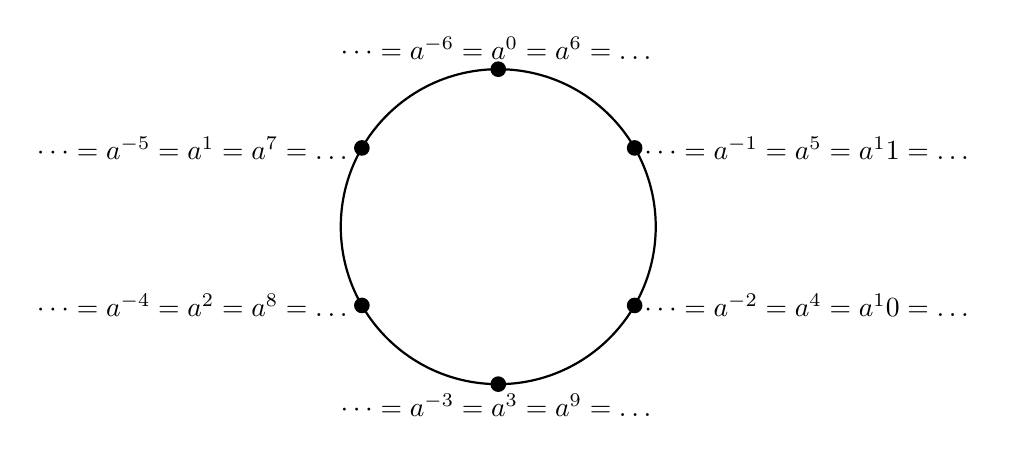
\begin{tikzpicture}
			\draw[thick] (0,0) circle (2cm);
			
			\draw ({60*(2-1) + 30}:2cm) node[circle,fill,inner sep=2pt] (2) {} node[above] (2) {$ \dots = a^{-6} = a^0 = a^6 = \dots$};
			\draw ({60*(3-1) + 30}:2cm) node[circle,fill,inner sep=2pt] (3) {} node[left] (3) {$ \dots = a^{-5} = a^1 = a^7 = \dots$};
			\draw ({60*(4-1) + 30}:2cm) node[circle,fill,inner sep=2pt] (4) {} node[left] (4) {$ \dots = a^{-4} = a^2 = a^8 = \dots$};
			\draw ({60*(5-1) + 30}:2cm) node[circle,fill,inner sep=2pt] (5) {} node[below] (5) {$ \dots = a^{-3} = a^3 = a^9 = \dots$};
			\draw ({60*(0-1) + 30}:2cm) node[circle,fill,inner sep=2pt] (0) {} node[right] (0) {$ \dots = a^{-2} = a^4 = a^10 = \dots$};
			\draw ({60*(1-1) + 30}:2cm) node[circle,fill,inner sep=2pt] (1) {} node[right] (1) {$ \dots = a^{-1} = a^5 = a^11 = \dots$};
		\end{tikzpicture}	
	\end{center}
	
	For these reasons, the cyclic groups $Z_n$ and $Z$ serve as prototypes for all cyclic groups, and algebraists say that there is essentially only one cyclic group of each order. What is meant by this is that, although there may be many different sets of the form $\{ a^n \mid n \in Z \}$, there is essentially only one way to operate on these sets. Algebraists do not really care what the elements of a set are; they care only about the algebraic properties of the set- that is, the ways in which the elements of a set can be combined.\newline
	
	The next theorem provides a simple method for computing $|a^k|$ knowing only $|a|$, and its first corollary provides a simple way to tell when $\cent{a^i} = \cent{a^j}$.
	\subsection{$\cent{a^k} = \cent{a^{\text{gcd}(n,k)}}$}
	\tikz \node[theorem]
	{
		\textbf{Theorem.} Let $a$ be an element of order $n$ in a group and let $k$ be a positive integer. Then $\cent{a^k} = \cent{a^{\text{gcd}(n,k)}}$ and $|a^k| = \frac{n}{\text{gcd}(n,k)}$
	};\newline
	
	\tikz \node[proof1]
	{
		\textbf{Proof.} To simplify the notation, let $d =$ gcd$(n,k)$ and let $k = dr$. Since $a^k = a^{dr} = (a^d)^r$, we have by clouse that $\cent{a^k} \subseteq \cent{a^d}$. By the gcd theorem, there are integers $s$ and $t$ such that $d = ns + kt$. So, $a^d = a^{ns+kt} = a^{ns}a^{kt} = (a^n)^sa^{kt} = e(a^k)^t = (a^k)^t \in \cent{a^k}$. This proves $\cent{a^d} \subseteq \cent{a^k}$. So, we have verified that $\cent{a^k} = \cent{a^{\text{gcd}(n,k)}}$.\newline
		
		We prove the second part of the theorem by showing first that $|a^d| = \frac{n}{d}$ for any divisor $d$ of $n$.
	};
	
	\tikz \node[proof]
	{
		 Clearly, $(a^d)^{n/d} = a^n = e$, so that $|a^d| \leq \frac{n}{d}$. On the other hand, if $i$ is a positive integer less then $\frac{n}{d}$, then $(a^d)^i \neq e$ by definition of $|a|$. We now apply this fact with $d =$ gcd$(n,k)$ to obtain $|a^k| = |\cent{a^k}| = |\cent{a^{\text{gcd}(n,k)}}|= |a^{\text{gcd}(n,k)}| = \frac{n}{\text{gcd}(n,k)}$.
	};\newline
	
	The advantage of the $4.2$ theorem is that it allows us to replace one generator of a cyclic subgroup with a more convenient one. For example, if $|a| = 30$, we have $\cent{a^{26}} = \cent{a^2}, \, \cent{a^{22}} = \cent{a^2}, \, \cent{a^{21}} = \cent{a^3}$. From this we can easily see that $|a^{23}| = 30$ and $|a^{22}| = 15$. Moreover, if one wants to list the elements of, say, $\cent{a^{21}}$, it is easier to list the elements of $\cent{a^3}$ instead. Theorem $4.2$ establishes an important relationship between the order of an element in a finite cyclic group and the order of the group.
	
	\subsubsection{Orders for elements in finite cyclic groups}
	\tikz \node[corollary]
	{
		\textbf{Corollary.} In a finity cyclic group, the order of an element divides the order of the group.
	};
	
	\subsubsection{Criterion for $\cent{a^i} = \cent{a^j}$ and $|a^i| = |a^j|$}
	\tikz \node[corollary]
	{
		\textbf{Corollary.} Let $|a| = n$. Then $\cent{a^i} = \cent{a^j}$ if and only if gcd$(n, \, j)$ = gcd$(n,i)$ and $|a^i| = |a^j|$ if and only if gcd$(n,\, j)$ = gcd$(n, \, i)$.
	};\newline
	
	\tikz \node[proof]
	{
		\textbf{Proof.} Theorem $4.2$ shows that $\cent{a^i} = \cent{a^{\text{gcd}(n, \, i)}}$ and $\cent{a^j} = \cent{a^{\text{gcd}(n, \, j)}}$, so that the proof reduces to proving that $\cent{a^{\text{gcd}(n, \, i)}} = \cent{a^{\text{gcd}(n, \, j)}}$ if and only if gcd$(n, \, i) =$ gcd$(n, \, j)$. Certainly, gcd$(n, \, i)$ = gcd$(n, \, j)$ implies that $\cent{a^{\text{gcd}(n, \, i)}} = \cent{a^{\text{gcd}(n, \, j)}}$. On the other hand, $\cent{a^{\text{gcd}(n, \, i)}} = \cent{a^{\text{gcd}(n, \, j)}}$ implies that $|a^{\text{gcd}(n, \, i)}| = |a^{\text{gcd}(n, \, j)}|$, so that by the second conclusion of Theorem $4.2$, we have $n / \text{gcd}(n, \, i) = n / \text{gcd}(n, \, j)$, and therefor gcd$(n, \, i)$ = gcd$(n, \, j)$.
	};
	
	\subsection{Generators of finite cyclic groups}
	\tikz \node[corollary]
	{
		\textbf{Corollary.} Let $|a| = n$. Then $\cent{a} = \cent{a^j}$ if and only if gcd$(n, \, j) = 1$ and $|a| = |\cent{a^j}|$ if and only if gcd$(n, \, j) = 1$.
	};
	
	\subsubsection{Generators of $Z_n$}
	\tikz \node[corollary]
	{
		\textbf{Corollary.} An integer $k$ in $Z_n$ is a generator of $Z_n$ if and only if gcd$(n, \, k) = 1$.
	};
	
	\subsection{Classification of subgroups of cyclic groups}
	\subsubsection{Fundamental theorem of cyclic groups}
	\tikz \node[theorem]
	{
		\textbf{Theorem.} Every subgroups of a cyclic groups is cyclic. Moreover, if $|\cent{a}| = n$, then the order of any subgroup of $\cent{a}$ is a divisor of $n$; and, for each positive divisor $k$ of $n$, the group $\cent{a}$ has exactly one subgroup of order $k$, namely, $\cent{a^{\frac{n}{k}}}$.
	};\newline
	
	Before we prove this theorem, let's see what it means. Suppose $G = \cent{a}$ and $G$ has order $30$. The first and second parts of the theorem say that if $H$ is any subgroup of $G$, then $H$ has the form $\cent{a^{\frac{30}{k}}}$ for some $k$ that is divisor of $30$. The third part of the theorem says that $G$ has one subgroup of each of the orders 1, 2, 3, 5, 6, 10, 15, and 30-and no others. The proof will also show how to find these subgroups.
	
	\tikz \node[proof]
	{
		\textbf{Proof.} Let $G = \cent{a}$ and suppose that $H$ is a subgroup of $G$. We must show that $H$ is cyclic. If it consists of the identity alone, then clearly $H$ is cyclic. So we may assume that $H \neq \{ e\}$. We now claim that, $H$ contains an element of the form $a^t$, where $t$ is positive. Since $G = \cent{a}$, every element of $H$ has the form of $a^t$; and when $a^t$ belongs to $H$ with $t < 0$, then $a^{-t}$ belongs to $H$ also and $-t$ is positive. Thus, our claim is verified. Now let $m$ be the least positive integer such that $a^m \in H$. By closure, $\cent{a^m} \subseteq H$. We next claim that $H = \cent{a^m}$. To prove this claim, if suffices to let $b$ be an arbitrary member of $H$ and show that $b$ is in $\cent{a^m}$. Since $b \in G = \cent{a}$, we have $b = a^k$ for some $k$. Now, apply the division algorithm to $k$ and $m$ to obtain integers $q$ and $r$ such that $k = mq + r$ where $0 \leq r < m$. Then $a^k = a^{mq + r} = a^{mq}a^r$, so that $a^r = a^{-mq}a^k$. Since $a^k = b \in H$ and $a^{-mq} = (a^m)^{-q}$ is in $H$ also, $a^r \in H$. But, $m$ is the least positive integer such that $a^m \in H$, and $0 \leq r < m$, so $r$ must be $0$. Therefore, $b = a^k = a^{mq} = (a^m)^q \in \cent{a^m}$. This proves the assertion of the theorem that every subgroup of a cyclic group is cyclic.\newline
		
		To prove the next portion of the theorem, suppose that $|\cent{a}| = n$ and $H$ is any subgroup of $\cent{a}$. We have already shown that $H = \cent{a^m}$, where $m$ is the least positive integer such that $a^m \in H$. Using $e = b = a^n$ as in the preceding paragraph, we have $n = mq$.\newline
		
		Finally, let $k$ be any positive divisor of $n$. We will show that $\cent{a^{\frac{n}{k}}}$ is the one and only subgroup of $\cent{a}$ order $k$. From Theorem $4.2$ we see that $\cent{a^{\frac{n}{k}}}$ has order $\frac{n}{\text{gcd}\left(n, \, \frac{n}{k}\right)} = \frac{n}{\frac{n}{k}} = k$. Now let $H$ be any subgroup of $\cent{a}$ order $k$. We have already shown above that $H = \cent{a^m}$, where $m$ is a divisor of $n$. Then $m = \text{gcd}(n, \, m)$ and $k = |a^m| = |a^{\text{gcd}(n, \, m)}| = \frac{n}{\text{gcd}(n, \, m)} = \frac{n}{m}$. Thus, $m = \frac{n}{k}$ and $H = \cent{a^{\frac{n}{k}}}$.
	};\newpage
	
	Returning for a moment to our discussion of the cyclic group $\cent{a}$, where $a$ has order 30, we may conclude from Theorem $4.3$ that the subgroups of $\cent{a}$ are precisely those of the form $\cent{a^m}$, where $m$ is a divisor of 30. Moreover, if $k$ is a divisor of 30, the subgroup of order $k$ is $\cent{a^\frac{30}{k}}$. So the list of subgroups of $\cent{a}$ is:
	
	\[
		\begin{array}{ll}
			\cent{a} = \{ e, \, a, \, a^2, \, \dots, \, a^{30} \} & |a| = |\cent{a}| = 30, \\
			\cent{a^2} = \{ e, \, a^2, \, a^4, \, \dots, \, a^{28} \} & |a^2| = |\cent{a^2}| = 15, \\
			\cent{a^3} = \{ e, \, a^3, \, a^6, \, \dots, \, a^{27} \} & |a^3| = |\cent{a^3}| = 10, \\
			\multicolumn{1}{c}{\vdots} & \multicolumn{1}{c}{\vdots} \\
			\cent{a^{15}} = \{ e, \, a^{15} \} & |a^{15}| = |\cent{a^{15}}| = 2, \\
			\cent{a^{30}} = \{ e \} & |a^{30}| = |\cent{a^{30}}| = 1.
		\end{array}		
	\]
	
	 \subsubsection{Subgroups of $Z_n$}
	 \tikz \node[corollary]
	 {
	 	\textbf{Corollary.} For each positive divisor $k$ of $n$, the set $\cent{\frac{n}{k}}$ is the unique subgroup of $Z_n$ order $k$; moreover, these are the only subgroups of $Z_n$.
	 };\newline
	 
	 By combining Theorems $4.2$ and $4.3$, we can easily count the number of elements of each order in a finite cyclic group. For convenience, we introduce an important number-theoretic function called the \textit{Euler phi function}. Let $\phi(1) = 1$, and for any integer $n > 1$, let $\phi(n)$ denote the number of positive integers less than $n$ and relatively prime to $n$. Notice that by definition of the group $U(n), \, |U(n)| = \phi(n)$. The first 12 values of $\phi(n)$ are given in table below.
	 
	 \begin{center}
		\begin{tabular}{|l|c|c|c|c|c|c|c|c|c|c|c|c|}
			\hline
			$n$ & 1 & 2 & 3 & 4 & 5 & 6 & 7 & 8 & 9 & 10 & 11 & 12 \\
			\hline
			$\phi(n)$ & 1 & 1 & 2 & 2 & 4 & 2 & 6 & 4 & 6 & 4 & 10 & 4 \\
			\hline
		\end{tabular} 	
	 \end{center}
	 
	 \subsubsection{Number of elements of each order in a cyclic group}
	 \tikz \node[theorem]
	 {
	 	\textbf{Theorem.} If $d$ is a positive divisor of $n$, the number of elements of order $d$ in a cyclic group of order $n$ is $\phi(d)$.
	 };\newpage
	 
	 \tikz \node[proof]
	 {
	 	\textbf{Proof.} By Theorem $4.3$, the group has exactly one subgroup of order $d$- call it $\cent{b}$. Then every element of order $d$ also generates the subgroup $\cent{b}$ and, by Corollary $3$ of Theorem $4.2$, and element $b^k$ generates $\cent{b}$ if and only if gcd$(k, \, d) = 1$. The number of such elements is precisely $\phi(d)$.\newline
	 	
	 	\textbf{Comment.} Let $G$ be a cyclic group and $G = \cent{a}$. $n := |a| = |\cent{a}|$. Let $0 < d \mid n$. By Theorem $4.3$ $\cent{a}$ has exactly one subgroup of order $d$, that is $\cent{a^\frac{n}{d}}$. So $|a^\frac{n}{d}| = |\cent{a^\frac{n}{d}}| = d$. Let $\cent{b} := \cent{a^\frac{n}{d}}$. Every element of order $d$ in $\cent{a}$ also generates $\cent{b}$. So, all the elements of order $d$ in a are in $\cent{b}$, and are generators. We need to find the number of generators in $\cent{b}$.
	 };
	 
	 \subsection{Number of elements of order $d$ in a finite group}
	 \tikz \node[corollary]
	 {
	 	\textbf{Corollary.} In a finite group, the number of elements of order $d$ is divisible by $\phi(d)$.
	 };\newline
	 
	 \tikz \node[proof]
	 {
	 	\textbf{Proof.} If a finite group has no elements of order $d$, the statement is true, since $\phi(d)$ divides $0$. Now suppose that $a \in G$ and $|a| = d$. By Theorem $4.4$, we know that $\cent{a}$ has $\phi(d)$ elements of order $d$. If all elements of order $d$ in $G$ are in $\cent{a}$, we are done. So, suppose that there is an element $b$ in $G$ of order $d$ that is not in $\cent{a}$. Then, $\cent{b}$ also has $\phi(d)$ elements of order $d$. This means that we have found $2\phi(d)$ elements of order $d$. provided that $\cent{a}$ and $\cent{b}$ have no elements or order $d$ in common. If there is an element $c$ of order $d$ that belongs to both $\cent{a}$ and $\cent{b}$, then we have $\cent{a} = \cent{c} = \cent{b}$, so that $b \in \cent{a}$, which is contradiction. Continuing in this fashion, we see that the number of elements of order $d$ in a finite group is a multiple of $\phi(d)$.
	 };\newpage
	
	\section{Permutation groups}
	Wigner’s discovery about the electron permutation group was just the
	beginning. He and others found many similar applications and nowadays
	group theoretical methods—especially those involving characters and
	representations—pervade all branches of quantum mechanics.
	
	\subsection{Definition and notation}
	\subsubsection{Permutation of $A$, permutation group of $A$}
	\tikz \node[definition]
	{
		\textbf{Definition.} A \textit{permutation} of a set $A$ is a function from $A$ to $A$ that is both one-to-one and onto. A \textit{permutation group} of a set $A$ is a set of permutations of $A$ that forms a group under function composition.
	};\newline
	
	We will focus on the case where $A$ is finite. Furthermore, it is customary, as well as convenient, to take $A$ to be a set of the form $\{ 1, \, 2, \, 3, \, \dots, \, n \}$ for some positive integer $n$. Permutations of finite sets are usually given by an explicit listing of each element of the domain and its corresponding functional value. For example, we define a permutation $\alpha$ of the set $\{ 1, \, 2, \, 3, \, 4 \}$ by specifying
	\[
		\alpha(1) = 2, \quad \alpha(2) = 3, \quad \alpha(3) = 1, \quad \alpha(4) = 4.
	\]
	
	A more convenient way to express this correspodence is to write $\alpha$ in array form as
	\[
		\alpha = 
		\begin{bmatrix}
			1 & 2 & 3 & 4 \\
			2 & 3 & 1 & 4
		\end{bmatrix}.
	\]
	
	\textbf{Example. Symmetric group of $S_3$} Let $S_3$ denote the set of all one-to-one functions from $\{ 1, \, 2, \, 3 \}$ to itself. Then $S_3$, under function composition, is a group with six elements. The six elements are
	\[
		\varepsilon =
		\begin{bmatrix}
			1 & 2 & 3 \\
			1 & 2 & 3 
		\end{bmatrix},\quad
		\alpha =
		\begin{bmatrix}
			1 & 2 & 3 \\
			2 & 3 & 1
		\end{bmatrix},\quad
		\alpha^2 = 
		\begin{bmatrix}
			1 & 2 & 3 \\
			3 & 1 & 2 
		\end{bmatrix},\quad
	\]
	
	\[
	\beta = 
	\begin{bmatrix}
		1 & 2 & 3 \\
		1 & 3 & 2 
	\end{bmatrix},\quad
	\alpha\beta =
	\begin{bmatrix}
		1 & 2 & 3 \\
		2 & 1 & 3
	\end{bmatrix},\quad
	\alpha^2\beta = 
	\begin{bmatrix}
		1 & 2 & 3 \\
		3 & 2 & 1 
	\end{bmatrix}.\quad
	\]
	
	Note that
	\[
	\beta\alpha =
	\begin{bmatrix}
		1 & 2 & 3 \\
		3 & 2 & 1	
	\end{bmatrix}
	= \alpha^2\beta \neq \alpha\beta
	\], so that $S_3$ is non-Abelian.
	\newpage
	
	\subsection{Cycle notation}
	There is another notation commonly used to specify permutations. It is called \textit{cycle notation} and was first introduced by the great French mathematician Cauchy in 1815. Cycle notation has theoretical advantages in that certain important properties of the permutation can be readily determined when cycle notation is used.\newline
	
	Let us consider the permutation
	\[
		\alpha = 
		\begin{bmatrix}
			1 & 2 & 3 & 4 & 5 & 6 \\
			2 & 1 & 4 & 6 & 5 & 3
		\end{bmatrix}
	\]
	In cycle notation: (1, 2)(3, 4, 6)(5).\newline
	Second example:
	\[
		\beta = 
		\begin{bmatrix}
			1 & 2 & 3 & 4 & 5 & 6 \\
			5 & 3 & 1 & 6 & 2 & 4
		\end{bmatrix}.
	\]
	In cycle notation: (1, 5, 2, 3)(4, 6).\newline
	An expression of the form $(a_1, \, a_2, \, \dots, \, a_m)$ is called a \textit{cycle of length $m$} or an $m$-\textit{cycle}.
	
	\subsection{Properties of permutations}
	\subsubsection{Products of disjoint cycles}
	\tikz \node[theorem]
	{
		\textbf{Theorem.} Every permutation of a finite set can be written as a cycle or as a product of disjoint cycles.
	};\newline
	
	\tikz \node[proof1]
	{
		\textbf{Proof.} Let $\alpha$ be a permutation on $A = \{ 1, \, 2, \, \dots, \, n \}$. To write $\alpha$ in disjoint cycle form, we start by choosing any member of $A$, say $a_1$, and let
		\[
			a_2 = \alpha(a_1), \quad a_3 = \alpha(\alpha(a_1)) = \alpha^2(a_1),
		\]
		and so on, until we arrive at $a_1 = \alpha^m(a_1)$ for some $m$. We know that such $m$ exists because the sequence $a_1, \, \alpha(a_1), \alpha^2(a_1), \, \dots$ must be finite; so there must eventually be a repetition, say $\alpha^i(a_1) = \alpha^j(a_1)$ for some $i$ and $j$ with $i < j$. Then $a^1 = \alpha^m(a_1)$, where $m = j-i$. We express this relationship among $a_1, \, a_2, \, \dots, \, a_m$ as
		\[
			\alpha = (a_1, \, a_2, \, \dots, \, a_m) \, \cdots.
		\]
		The three dots at the end indicate the possibility that we may not have exhausted the set $A$ in this process. In such case, we merely choose any element $b_1$ of $A$ not appearing in the first cycle and proceed to create a new cycle before. That is, we let $b_2 = \alpha(b_1), \, b_3 = \alpha^2(b_1)$, and so on, until we reach $b_1 = \alpha^k(b_1)$ for some $k$. This new cycle will have no elements in common with the previously constructed cycle. For, if so, then $\alpha^i(a_1) = \alpha^k(b_1)$ for some $i$ and $j$. But then $\alpha^{i-j}(a_1) = b_1$, and therefore $b_1 = a_t$ for some $t$. 
	};
	
	\tikz \node[proof]
	{
		This contradicts the way $b_1$ was chosen. Continuing this process until we run out of elements of $A$, our permutation will appear as
		\[
		\alpha = (a_1, \, a_2, \, \dots, \, a_m)(b_1, \, b_2, \, \dots, \, b_k) \cdots (c_1, \, c_2, \, \dots, \, c_s).
		\]
		In this way, we see that every permutation can be written as a product of disjoint cycles.
	};
	
	\subsubsection{Disjoint cycles commute}
	\tikz \node[theorem]
	{
		If the pair of cycles $\alpha = (a_1, \, a_2, \, \dots, \, a_m)$ and $\beta = (b_1, \, b_2, \, \dots, \, b_n)$ have no entries in common, then $\alpha\beta = \beta\alpha$.
	};\newline
	
	\tikz \node[proof]
	{
		\textbf{Proof.} For definiteness, let us say that $\alpha$ and $\beta$ are permutations of the set
		\[
			S = \{ a_1, \, a_2, \, \dots, \, a_m, \, b_1, \, b_2, \, \dots, \, c_1, \, c_2, \, \dots, \, c_k \}
		\]
		where the $c$'s are the members of $S$ left fixed by both $\alpha$ and $\beta$ (there may not be any $c$'s). To prove that $\alpha\beta = \beta\alpha$, we must show that $(\alpha\beta)(x) = (\beta\alpha)(x)$ for all $x$ in $S$. If $x$ is one of the $a$ elements, say $a_i$, then
		\[
			(\alpha\beta)(a_i) = \alpha(\beta(a_i)) = \alpha(a_i) = a_{i+1},
		\]
		since $\beta$ fixes all $a$ elements. (We interpret $a_{i+1}$ as $a_1$ if $i = m$.) For the same reason,
		\[
			(\beta\alpha)(a_i) = \beta(\alpha(a_i)) = \beta(a_{i+1}) = a_{i+1}.
		\]
		Hence, the functions of $\alpha\beta$ and $\beta\alpha$ agree on the $a$ elements. A similar argument shows that $\alpha\beta$ and $\beta\alpha$ agree on the $b$ elements as well. Finally, suppose that $x$ is a $c$ element, say $c_i$. Then, since both $\alpha$ and $\beta$ fix $c$ elements, we have
		\[
			(\alpha\beta)(c_i) = \alpha(\beta(c_i)) = \alpha(c_i) = c_i
		\]
		and
		\[
			(\beta\alpha)(c_i) = \beta(\alpha(c_i)) = \beta(c_i) = c_i.
		\]
		This completes the proof.
	};\newline
	
	The next theorem shows that the disjoint cycle form has the enormous advantage of allowing us to "eyeball" the order of the permutation.
	
	\subsubsection{Order of a permutation}
	\tikz \node[theorem]
	{
		\textbf{Theorem.} The order of a permutation of a finite set written in disjoint cycle form is the least common multiple of the lengths of the cycles.
	};\newline
	
	\tikz \node[proof]
	{
		\textbf{Proof.} First, observe that a cycle of length $n$ has order $n$.
		Let $G$ be a permutation group of the set $A = \{ 1, \, 2, \, 3, \, 4, \, 5 \}$ and $\alpha \in G$.
		\[
			\alpha =
			\begin{bmatrix}
				1 & 2 & 3 & 4 & 5 \\
				3 & 1 & 2 & 5 & 4
			\end{bmatrix}
		\]
		In disjoint cycle form: $\alpha = (132)(45)$.\newline
		$\alpha$ can be written as $\alpha' \circ \alpha''$ or $\alpha'' \circ \alpha'$, where
		\[
			\alpha' =
			\begin{bmatrix}
				1 & 2 & 3 & 4 & 5 \\
				3 & 1 & 2 & 4 & 5
			\end{bmatrix}, \quad
			\alpha'' =
			\begin{bmatrix}
				1 & 2 & 3 & 4 & 5 \\
				1 & 2 & 3 & 5 & 4
			\end{bmatrix}
		\]
		$\alpha' = (132), \, \alpha'' = (45)$.
		Let us see the order of these functions:
		\[
			(\alpha')^1 = 
			\begin{bmatrix}
				1 & 2 & 3 & 4 & 5 \\
				3 & 1 & 2 & 4 & 5
			\end{bmatrix}, \quad
			(\alpha')^2 = 
			\begin{bmatrix}
				1 & 2 & 3 & 4 & 5 \\
				2 & 3 & 1 & 4 & 5
			\end{bmatrix}, \quad
			(\alpha')^3 = 
			\begin{bmatrix}
				1 & 2 & 3 & 4 & 5 \\
				1 & 2 & 3 & 4 & 5
			\end{bmatrix}.
		\]
		\[
			(\alpha'')^1 = 
			\begin{bmatrix}
				1 & 2 & 3 & 4 & 5 \\
				1 & 2 & 3 & 5 & 4
			\end{bmatrix}, \quad
			(\alpha'')^2 = 
			\begin{bmatrix}
				1 & 2 & 3 & 4 & 5 \\
				1 & 2 & 3 & 4 & 5
			\end{bmatrix}.
		\]
		We can see that $|\alpha'| = 3, \, |\alpha''| = 2$, that are equal with the lengths of the cycles.\newline
		
		Next, suppose that $\alpha$ and $\beta$ are disjoint cycles of lengths $m$ and $n$, and let $k$ be the least common multiple of $m$ and $n$. It follows from Theorem $4.1$ that both $\alpha^k$ amd $\beta^k$ are the identity permutation $\mathcal{E}$ ($\alpha^m = \alpha^k \Longleftrightarrow m \mid m - k$) and, since $\alpha$ and $\beta$ commute, $(\alpha\beta)^k = \alpha^k\beta^k$ is also the identity. Thus, we know by Corollary 2 to Theorem $4.1$ ($a^k = e \Longleftrightarrow |a| \mid k$) that the order of $\alpha\beta$ -let us call it $t$- must divide $k$. But then $(\alpha\beta)^t = \alpha^t\beta^t = \mathcal{E}$, so that $\alpha^t = \beta^{-t}$. However, it is clear that if $\alpha$ and $\beta$ have no common symbol, the same is true for $\alpha^t$ and $\beta^{-t}$, since raising a cycle to a power does not introduce new symbols. But if $\alpha^t$ and $\beta^{-t}$ are equal and have no common symbol, they must both be the identity, because every symbol in $\alpha^t$ is fixed by $\beta^{-t}$ and vice versa. It follows, then, that both $m$ and $n$ divides $t$ also. ($\alpha^t = e \Longleftrightarrow m \mid t$). This means that $k$, the least common multiple of $m$ and $n$, divides $t$ also. This shows that $k = t$.\newline
		
		Thus far, we have proved that the theorem is true in the cases where the permutation is a single cycle or a product of two disjoint cycles. The general case involving more than two cycles can be handled in an analogous way.
	};\newline
	
	As we will soon see, a particularly important kind of permutation is a cycle of length 2-that is, a permutation of the form $(ab)$ where $a \neq b$. Many authors call these permutations \textit{transpositions}, since the effect of $(ab)$ is to interchange or transpose $a$ and $b$.
	
	\subsubsection{Product of 2-cycles}
	\tikz \node[theorem]
	{
		\textbf{Theorem.} Every permutation in $S_n, \, n > 1$, is a product of 2-cycles.
	};\newline
	
	\tikz \node[proof]
	{
		\textbf{Proof.} First, note that the identity can be expressed as (12)(12), and it is a product of 2-cycles. By Theorem $5.1$, we know that every permutation can be written in the form
		\[
			(a_1a_2 \cdots a_k)(b_1b_2\cdots b_t) \cdots (c_1c_2 \cdots c_s).
		\]
		A direct computation shows that this is the same as
		\[
			(a_1a_k)(a_1a_{k-1})\cdots(a_1a_2)(b_1b_t)(b_1b_{t-1})\cdots(b_1b_2)(c_1c_s)(c_1c_{s-1})\cdots(c_1c_2).
		\]
		This completes the proof.
	};\newline
	
	\textbf{Example.}
	\[
		(12345) = (15)(14)(13)(12)
	\]
	\[
		(1632)(457) = (12)(13)(16)(47)(45)
	\]
	The decomposition of a permutation into a product of 2-cycles given in the proof of Theorem $5.4$ is not the only way a permutation can be written as a product of 2-cycles. Although the next example shows that even the \textit{number} of 2-cycles may vary from one decomposition to another, we will prove in Theorem $5.5$ (first proved by Cauchy) that there is one aspect of a decomposition that never varies.\newline
	
	We isolate a special case of Theorem $5.5$ as a lemma.\newline
	
	\tikz \node[theorem]
	{
		\textbf{Lemma.} If $\mathcal{E} = \beta_1\beta_2\cdots \beta_r$, where the $\beta$'s are 2-cycles, then $r$ is even.
	};\newline
	
	\tikz \node[proof1]
	{
		\textbf{Proof.} Clearly, $r \neq 1$, since a 2-cycle is not the identity. If $r = 2$, we are done. So, we suppose that $r > 2$, and we proceed by induction. Since $(ij) = (ji)$, the product $\beta_{r-1}\beta_r$ can be expressed in one of the following forms shown on the right:
	};
	
	\tikz \node[proof]
	{
		\[
		\mathcal{E} = (ab)(ab)
		\]
		\[
		(ab)(bc) = (ac)(ab)
		\]
		\[
		(ac)(cb) = (bc)(ab)
		\]
		\[
		(ab)(cd) = (cd)(ab).
		\]
		If the first case occurs, we may delete $\beta_{r-1}\beta_r$ from the original product to obtain $\mathcal{E} = \beta_1\beta_2 \cdots \beta_{r-2}$. In the other three cases, we replace the form of $\beta_{r-1}\beta_r$ on the right by its counterpart in the left to obtain a new product of $r$ 2-cycles that is still the identity, but where the rightmost occurence of the integer $a$ is in the second-from-the-rightmost 2-cycle of the product instead of the rightmost 2-cycle. We now repeat the procedure just described with $\beta_{r-2}\beta_{r-1}$, and, as before, we obtain a product of $(r-2)$ 2-cycles equal to the identity or a new product of $r$ 2-cycles, where the rightmost occurence of $a$ is in the third 2-cycle from the right. Continuing this process, we must obtain a product of $(r-2)$ 2-cycles equal to the identity, because otherwise we have a product equal to the identity in which the only occurence of the integer $a$ is in the leftmost 2-cycle, and such product does not fix $a$, whereas the identity does. Hence, by the \textit{Second principle of mathematical induction}, $r-2$ is even, and $r$ is even as well.
	};
	
	\subsubsection{Always even or always odd}
	\tikz \node[theorem]
	{
		\textbf{Theorem.} If a permutation $\alpha$ can be expressed as a product of an even (odd) number of 2-cycles, then every decomposition of $\alpha$ into a product of 2-cycles must have an even (odd) number of 2-cycles. In symbols, if
		\[
			\alpha = \beta_1\beta_2 \cdots \beta_r \quad \text{and} \quad \alpha = \gamma_1\gamma_2 \cdots \gamma_s,
		\]
		where the $\beta$'s and the $\gamma$'s are 2-cycles, then $r$ and $s$ are both even or both odd.
	};\newline
	
	\tikz \node[proof]
	{
		\textbf{Proof.} Observe that $\beta_1\beta_2 \cdots \beta_r = \gamma_1\gamma_2 \cdots \gamma_s$ implies
		\[
			\mathcal{E} = \gamma_1\gamma_2 \cdots \gamma_s \beta_1^{-1}\beta_2^{-1} \cdots \beta_r^{-1} = \gamma_1\gamma_2 \cdots \gamma_s \beta_1\beta_2 \cdots \beta_r
		\]
		since a 2-cycle is its own inverse. Thus, the lemma on page 104 guarantees that $s+r$ is even. It follows that $r$ and $s$ are both even or both odd.
	};
	
	\subsubsection{Even and odd permutations}
	\tikz \node[definition]
	{
		\textbf{Definition.} A permutation that can be expressed as a product of an even number of 2-cycles is called an \textit{even permutation}. A permutation that can be expressed as a product of an odd number of 2-cycles is called an \textit{odd permutation}.
	};\newline
	
	Theorems $5.4$ and $5.5$ together show that every permutation can be unambigously classified as either even or odd. The significance of this observation is given in Theorem $5.6$.
	
	\subsubsection{Even permutations form a group}
	\tikz \node[theorem]
	{
		\textbf{Theorem.} The set of even permutations in $S_n$ forms a subgroup of $S_n$.
	};\newline
	
	\tikz \node[proof]
	{
		\textbf{Proof.} This proof is left to the reader.
	};
	
	\subsubsection{Alternating group of degree $n$}
	\tikz \node[definition]
	{
		\textbf{Definition.} The group of even permutations of $n$ symbols is denoted by $A_n$ and is called the \textit{alternating group of degree $n$}.
	};
	
	\subsubsection{Order of the alternating group of degree $n$}
	\tikz \node[theorem]
	{
		\textbf{Theorem.} For $n > 1, \, A_n$ has order $\frac{n!}{2}$.
	};\newline
	
	\tikz \node[proof]
	{
		\textbf{Proof.} For each odd permutation $\alpha$, the permutation $(12)\alpha$ is even and $(12)\alpha \neq (12)\beta$ when $\alpha \neq \beta$. Thus, there are at least as many even permutation as there are odd ones. On the other hand, for each even permutation $\alpha$, the permutation $(12)\alpha$ is odd and $(12)\alpha \neq (12)\beta$ when $\alpha \neq \beta$. Thus, there are at least as many odd permutations as there are even ones. It follows that there are equal members of even and odd permutations. Since $|S_n| = n!$, we have $|A_n| = \frac{n!}{2}$.
	};

\end{document}